In this chapter we present the SMT problem. Recall that our goal is to translate proofs of unsatisfiability of SMT queries into Lean proofs. Therefore, besides presenting formally the problem and explaining how it is solved, we focus on showing how proofs are represented in an SMT solver.

\subsection{Description of the Problem}

The Boolean Satisfiability Problem (SAT) consists in determining whether a formula in Propositional Logic (PL), which contains free variables, can be evaluated as \textit{true} by finding a function that assigns Boolean values to each variable.
We say that a formula is satisfiable if such a function exists, and unsatisfiable otherwise. In
this work, we will be focusing on the problem CNF-SAT, an equivalent version of SAT in
which the input formula always comes in Conjunctive Normal Form, that is, a conjunction
of disjunctions of literals. From now on, we will use SAT to refer to the CNF-SAT problem. Besides that, we will write \textit{clause} to refer to each one of the disjunctions in some
input formula for SAT.\ We will also treat a clause as a set of its composing literals and use set operations over it. For instance, we will write $x \in C$ to state that the literal $x$ is present in clause $C$ and $C \setminus \{x\}$ to refer to the clause $C$ without the literal $x$.


Satisfiability Modulo Theories (SMT)~\cite{smt} is a generalization of SAT.\
There are two additions: first, the underlying logic framework is First Order
Logic (FOL) instead of Propositional Logic. This means that the input formula
can contain quantifiers binding variables, unintepreted function symbols,
predicates asserting properties about variables and a special symbol ``$\simeq$'' that is used to assert equality between terms. %\sout{and an arbitrary domain from which the variables can be drawn.} \tom{I think it's better to not talk about domains here (?) It may be confusing since we are adding them again with the second addition. I am not trying to define precisely first order logic (should I?), just informally saying what are the additions}
The second addition is the inclusion of a set of theories that
allows the problem to refer to variables of different types. More
precisely, a theory consists of a sort (for instance, integers) over which a
subset of the variables of the problem can range over and a set of symbols
that represents operations over terms of these sorts with predefined semantics (for
instance, addition and comparison operations over integers). Instances of the
problem are allowed to use multiple theories at the same time. The logic
framework that corresponds to Propositional Logic with these two additions is
known as Many-Sorted First Order Logic (MSFOL). The precise syntax and semantics of this logic framework
is given in detail for example in~\cite{many_sorted}. In
Section~\ref{sec:msfolHere} we give a brief overview of it.

\subsection{Many-Sorted First Order Logic}\label{sec:msfolHere}
\subsubsection{Syntax}

The syntax of MSFOL consists of three syntatic categories:

\begin{enumerate}
  \item \textbf{Sorts}. Symbols identifying the kinds of variables that are allowed. They are defined by the following grammar:
        \begin{center}
          $ \tau ::= \sigma \mid (\tau_{1}, \tau_{2}, \ldots, \tau_{n}) \rightarrow \tau$ % \mid (\tau_{1}, \tau_{2}, \ldots, \tau_{m})$
        \end{center}
        The first case represents an atomic sort drawn from a predefined set of sorts, which we will refer to as $\mathcal{S}_{S}$, and is required to have a cardinality that is at most countably infinite. The second case represents sorts of functions with arity $n$. We will always assume that there is a special sort in $\mathcal{S}_{S}$ named $\textit{bool}$.
  \item \textbf{Terms}. Symbols representing sorted variables, constants or function applications. Function applications are only well formed when the sorts are respected. The symbols annotated on top of each term represent their sort, and they will be ommited when they can be inferred.
        \begin{center}
          $ t ::= x^{\tau} \mid f^{(\tau_{1}, \ldots, \tau_{n}) \rightarrow \tau}(t_{1}, \dots, t_{n}) $
        \end{center}
        Function symbols are also drawn from a predefined set, which we will refer to as $\mathcal{S}_{F}$, and it is also required to have a cardinality that is at most countably infinite. Constants are represented by nullary functions. Terms will also be referred to as ``atoms''. We will use the term ``predicate'' to refer to functions whose return type is $\textit{bool}$. Variables, when not binded by a quantifier, will also be drawn from a predefined set, which we will refer to as $\mathcal{S}_{X}$ and, again, impose the requirement of having a cardinality that is at most countably infinite.
  \item \textbf{Formulas}. Symbols representing boolean expressions, possibly involving terms.
        \begin{center}
          $ \psi ::= \psi_{1} \vee \psi_{2} \mid \forall x.\psi \mid \neg \psi \mid \psi_{1} \simeq \psi_{2}$
        \end{center}
\end{enumerate}

We also define the following symbols:

\begin{center}
  $\exists x. \psi := \neg \forall x. \neg \psi$\\
  $\psi_{1} \wedge \psi_{2} := \neg (\neg \psi_{1} \vee \neg \psi_{2})$\\
  $\psi_{1} \rightarrow \psi_{2} := \neg \psi_{1} \vee \psi_{2}$\\
  $\psi_{1} \leftrightarrow \psi_{2} := \psi_{1} \Rightarrow \psi_{2} \wedge \psi_{2} \Rightarrow \psi_{1}$\\
  $\psi_{1} \not\simeq \psi_{2} := \neg (\psi_{1} \simeq \psi_{2})$
\end{center}

We define a \textit{signature} to be a triple of sets $\langle \mathcal{S}_{S}, \mathcal{S}_{F}, \mathcal{S}_{X} \rangle$ respecting the requirements defined above.

\subsubsection{Semantics}

Having established how terms in MSFOL are built, we have to define how they are evaluated and what is their meaning.
Given a signature $\Sigma = \langle \mathcal{S}_{S}, \mathcal{S}_{F}, \mathcal{S}_{X} \rangle$, a $\Sigma$\textit{-structure} is an assignemnt that matches, for each sort symbol $s \in \mathcal{S}_{S}$, a corresponding set $D_{s}$, and, for each function symbol $f^{\tau_{1}, \ldots, \tau^{n} \rightarrow \tau} \in \mathcal{S}_{F}$, a function $D_{f}$ of type $D_{\tau_{1}} \times \cdots \times D_{\tau_{n}} \rightarrow D_{\tau}$.
The $\textit{bool}$ sort will always be matched with the usual set of Boolean values, and the set $\mathcal{S}_{F}$ will always contain two nullary functions $\textit{true}$ and $\textit{false}$ which will be matched with the usual true and false values, represented here respectively as $true^{I}$ and $false^{I}$. We will also use the name \textit{Theory} as a synonym of structure.

\begin{example}[LIA]\label{ex:lia}
  Let $\mathcal{S}_{S} := \{Z\}$, $\mathcal{S}_{F} := \{add, sub, zero, succ, pred, lt\}$ and
  $S_{X} := \{x, y\}$. Examples of formulas that can be written using the signature composed by these sets include ``$lt(sub(x, y), succ(zero))$'' and ``$add(x, y) \simeq add(y, x)$''. For this particular signature, we can have many structures. For instance, by letting $D_{Z} := \mathbb{Z}$ and matching each function symbol to its natural operation over integers, we have a structure that represents formulas over integer numbers. On the other hand, if we let $D_{Z} := \mathbb{Z}_{13}$ and match each function symbol with the corresponding operation over integers modulo $13$, we have a structure representing formulas over integers modulo $13$. In the first case, the presented structure is known as \textit{LIA} (standing for Linear Integer Arithmetic).
\end{example}

Given a signature $\Sigma = \langle \mathcal{S}_{S}, \mathcal{S}_{F}, \mathcal{S}_{X} \rangle$, an \textit{Interpretation} is a $\Sigma$-structure paired with an interpretation function $\mathcal{I}$, which assigns to each free variable $x \in \mathcal{S}_{X}$ of sort $s$ a value in $D_{s}$. We denote by $\mathcal{I}_{x \gets v}$ the extension of the function $\mathcal{I}$ that also assigns the value $v$ to the variable $x$. Finally, we define the \textit{Evaluation} of a given formula $\psi$ over an interpretation $\mathcal{I}$, denoted by $\llbracket \psi \rrbracket^{\mathcal{I}}$, in the following way:
\begin{align*}
  \llbracket x \rrbracket^{\mathcal{I}} &:= \mathcal{I}(x) \\
  \llbracket f(t_{1}, \ldots, t_{n}) \rrbracket^{\mathcal{I}} &:= D_{f}(\llbracket t_{1} \rrbracket^{\mathcal{I}}, \ldots, \llbracket t_{n} \rrbracket^{\mathcal{I}}) \\
  \llbracket \bot \rrbracket &:= false^{I} \\
  \llbracket t_{1} \simeq t_{2} \rrbracket^{\mathcal{I}} &:= \llbracket t_{1} \rrbracket^{\mathcal{I}} = \llbracket t_{2} \rrbracket^{\mathcal{I}} \\
  \llbracket \neg \psi \rrbracket^{\mathcal{I}} &:= \llbracket \psi \rrbracket^{\mathcal{I}} = false^{I} \\
  \llbracket \psi_{1} \vee \psi_{2} \rrbracket^{\mathcal{I}} &:= \llbracket \psi_{1} \rrbracket^{\mathcal{I}} = true^{I}\,\, or\,\, \llbracket \psi_{2} \rrbracket^{\mathcal{I}} = true^{I} \\
  \llbracket \forall x . \psi \rrbracket^{\mathcal{I}} &:= \llbracket \psi \rrbracket^{\mathcal{I}_{x \gets v}} = true^{I} \text{, for any } v
\end{align*}

We say that an interpretation $\mathcal{I}$ \textit{satisfies} a formula $\psi$ if and only if $\mathcal{I}(\psi) = true^{I}$. If there is at least
one interpretation that satisfies a given formula $\psi$, it is said to be \textit{satisfiable}, otherwise it is $\textit{unsatisfiable}$.


\subsection{SMT Solvers}

An SMT solver is a piece of software whose main goal is to solve the SMT problem. Many-Sorted First Order Logic is undecidable in its most general form~\cite{fol_undec}, therefore SMT solvers have to limit themselves to use heuristics to solve a subset of the instances of the problem. In this section we present the ideas used by these systems that are more relevant to the present work.

\subsubsection{Davis–Putnam–Logemann–Loveland Algorithm (DPLL)}

First, let’s explore how SAT is solved. Although MSFOL is not decidable, Propositional Logic is, therefore, it is possible to design a decision procedure for SAT.\@ Indeed, one simple way to check whether a formula in PL with $n$ variables is satisfiable or not is to simply test each one of the $2^{n}$ functions assigning truth values to those variables.

A more efficient alternative of a decision procedure for PL is the DPLL algorithm~\cite{dpll}. DPLL is based on the \textit{Resolution} theorem:

\begin{theorem}[Resolution]\label{res_theorem}
Let $x$ be a literal. Let $C_{1}$ and $C_{2}$ be two clauses such that $x \in C_{1}$ and $\neg x \in C_{2}$. Then $C_{1} \wedge C_{2} \rightarrow (C_{1} \setminus x) \vee (C_{2} \setminus \neg x)$.
\end{theorem}

More specifically, it is based on \textit{Unit Resolution} (UR), that is, a more restricted version of resolution in which $C_{1} = \{x\}$ or $C_{2} = \{\neg x\}$. Notice that the clause that is inferred from the unit resolution theorem is equal to one of the clauses in the premisses, with one less literal. The general idea of the DPLL algorithm is to explore this fact to generate smaller clauses, while this is possible. Once all possible unit resolutions are performed, the algorithm makes a decision, assigning a boolean value to a variable. This action can potentially create more clauses suitable for unit resolution, which will be then explored. If this decision do not lead to the conclusion that the original formula is satisfiable, the procedure backtracks and assign the variable to the other boolean value. If this decision also does not lead to a positive conclusion, then the original formula is unsatisfiable.

\begin{figure}[t]
% \textbf{Input:} $\psi$, a PL formula\\
% \textbf{Output:} \textit{true} or \textit{false}, depending whether $\psi$ is satisfiable
\begin{algorithmic}[1]
\Function{SolvePL}{$\psi$}
\State $\psi \gets \Call{ConvertCNF}{\psi}$
\If{$\exists C \in \psi .\, C = \{\} \vee C = \{\bot\}$}
  \State \Return~\textit{false}
\ElsIf{$\forall C \in \psi .\, \top \in C$}
  \State \Return~\textit{true}
\Else
  \If{$\exists x \in \mathit{Vars}(\psi) \,$ such that $x$ is a target for UR}
    \State $\langle C_{1}, C_{2} \rangle \gets$ \Call{findClauses}{$x$, $\psi$} \Comment{Suitable for applying UR with $x$}
    \State~\Return~\Call{SolvePL}{$\psi \wedge C_{1} \diamond_{x} C_{2}$}
  \Else
    \State~Let $x$ be an unassinged variable in $\psi$
    \State~\Return~\Call{SolvePL}{$\psi_{\{x \gets \top\}}$} $\vee$ \Call{SolvePL}{$\psi_{\{x \gets \bot\}}$}
  \EndIf
\EndIf
\EndFunction
\end{algorithmic}
\caption{DPLL Algorithm}~\label{dpllAlgo}
\end{figure}

Figure~\ref{dpllAlgo} shows an implementation of this idea. The procedure \textit{SolvePL} works as follows: first, in lines 3 to 6, it checks if the formula can be evaluated to \textit{true} or \textit{false}. In case it is not possible, the procedure finds as many variables in which it can apply Unit Resolution as possible using the routine \textit{findClauses} and invokes itself recursively with each new application found, as shown in lines 8 to 10. By the resolution theorem, the formula that will be used as a parameter in the recursive call is satisfiable if and only if the one that was received by input is also satisfiable, therefore, this step is sound. Once there are no more possibilities, it chooses an arbitrary variable and make two recursive calls in line 13: one assigning this variable to \textit{true} and the other one to \textit{false}. Since these are the only two possibilities for that variable, the input formula is satisfiable if and only if one of the recursive calls returned \textit{true}. The algorithm uses this information to correctly return the disjunction between the two return values.

The actual algorithm used by most SMT solvers to solve SAT is a refinement over DPLL, called known as Conflict Driven Clause Learning (CDCL)~\cite{cdcl}. Its main idea is to modify the algorithm so that, when it finds a conflict (an empty clause or a clause that only contains false variables), analyze the reason for this conflict, allowing it to derive new clauses and to backtrack many decisions of values of variables at once. Since this refinement is not relevant for this work, we will not present it in detail here.

\subsubsection{CDCL(T)}

Assuming that we have a decision procedure for a given theory (or a combination of them), we can use it to extend the CDCL algorithm for checking the satisfiability of MSFOL formulas involving that theory. In this section we will study the CDCL(T)~\cite{cdcl_t} framework, that is a method for doing this extension over CDCL.\

\begin{figure}[t]
% \textbf{Input:} $\psi$, a formula in MSFOL over a theory  $\mathcal{T}$ \\
% \textbf{Output:} \textit{true} or \textit{false}, depending whether $\psi$ is satisfiable
\begin{algorithmic}[1]
\Function{SolveMSFOL}{$\psi$}
\State $\psi' \gets \Call{Convert}{\psi}$ \Comment{Get PL formula from MSFOL formula}
\If{$\Call{CDCL}{\psi'}$}
  \State $\mathcal{I} \gets \Call{GetInterpretation}{\psi'}$
  \If{$\Call{TheorySolver}{\mathcal{I}, \psi}$} \Comment{Check if $\mathcal{I}$ is compatible with $\psi$}
    \State~\Return \textit{true}
  \Else
    \State $L \gets \Call{GetConflictingLemma}{\mathcal{I}, \psi}$
    \State~\Return $\Call{SolveMSFOL}{\psi \wedge L}$
  \EndIf
\Else
  \State~\Return \textit{false}
\EndIf
\EndFunction
\end{algorithmic}
\caption{CDCL(T) Algorithm}~\label{cdclTAlgo}
\end{figure}

Consider a formula $\psi$ over a theory $\mathcal{T}$ in MSFOL.\ Let's assume we have a solver for this theory (that is, a method for deciding whether a given set of propositions in $\mathcal{T}$ is consistent or not). The idea behind CDCL(T) is to create a PL formula $\psi'$ from $\psi$ by substituting each theory atom (that is, an atom that is not a subexpression of another atom in the original formula) in it for a fresh boolean variable. We can then use the previously described CDCL algorithm to determine whether $\psi'$ is satisfiable. For instance, consider $\psi$ to be the formula $x > 3 \wedge x < -2$. From it, we would generate the PL formula $p \wedge q$, where $p$ represents $x > 3$ and $q$ represents $x < -2$. If $\psi'$ is unsatisfiable, then $\psi$ is also unsatisfiable. If this was not the case, it would be possible for $\psi'$ be unsatisfiable and $\psi$ be satisfiable. This means that there would exist an interpretation for $\psi$ which yields the value true. From this interpretation, we would be able to derive truth values for the variables in $\psi'$ that should satisfy the formula, but this is an absurd since $\psi'$ is unsatisfiable.
If $\psi'$ is satisfiable, we can find a interpretation $\mathcal{I}$ for $\psi'$. Although $\mathcal{I}$ satisfies $\psi'$, it is possible that it contradicts some fact about $\mathcal{T}$. In our previous example,
the only possible interpretation satisfying $\psi'$ is the one that assigns $p$ and $q$ to $true^{I}$, but this is not valid when we translate back to $\psi$, as $x$ cannot be both greater than $3$ and smaller then $-2$.
 If this happens, we rely on the theory solver to provide a new lemma from $\mathcal{T}$ that shows why the previous assignment was invalid. In this case, it would provide the lemma $\neg (x > 3 \wedge x < -2)$. Note that we are assuming that our theory solver has the capability of producing such a conflicting lemma for a particular interpretation.


Figure~\ref{cdclTAlgo} shows an implementation of CDCL(T). The procedure \textit{SolveMSFOL} works as follows: first, in line 2, we perform the conversion that we just described, in order to obtain a PL formula. Then, in line 3, we run the procedure \textit{CDCL} to determine if $\psi'$ is satisfiable. In case it is not, we just return \textit{false} in line 12. Otherwise, there exists an interpretation $\mathcal{I}$ that satisfies $\psi'$. This interpretation is obtained in line 4 and we proceed to check if the theory solver accepts it for $\psi$ in line 5. If it does accept, the formula is definitely satisfiable and we can return \textit{true}, as done in line 6. Otherwise, the conflicting lemma for the given interpretation is generated in line 8. We then repeat this process in line 9, adding the conflicting lemma to $\psi$.

\subsubsection{Equality and Uninterpreted Functions}\label{sec:euf}

In this work, we will be interested in two theories and their respective solvers. The first one is Equality and Uninterpreted Functions.

Consider the following problem: given a set of variables and uninterpreted functions and a set of equalities built from variables and functions applied to those variables, decide whether a given equality is a consequence of the conjunction of the ones in the set. For instance, let $a$, $b$, $c$ and $d$ be variables and $f$ a function of arity $1$. For now we assume that all variables belong to an artificial sort $U$, and all functions take arguments from this sort. The set $S := \{b = c, f(b) = c, f(c) = a\}$ have as a consequence the equality $a = b$.

The set of all equalities that can be derived from a given set of equalities built from variables and function applications is known as the \textit{congruence closure} of that set. Deciding whether a given equality is in the congruence closure for a given set is an old problem, which was shown to be decidable by Ackermann in 1954~\cite{ack_cong}. It is also is used as the basis for the theory of Equality and Uninterpreted Functions (EUF) in SMT.\

Note that, since MSFOL already has a built-in equality operator, we can encode this problem in this language by simply defining a set $U^{I}$, which will correspond to the artificial sort $U$ and a set of variables $\mathcal{S}_{X}$ which will include all variables and functions that are going to be used in instances of the problem. The set $\mathcal{S}_{F}$ will be empty. Since this theory does not add any new function in MSFOL, it is also known as the ``empty theory''.

We now give a brief overview on the standard algorithm for finding the congruence closure of a given set of equalities. A more detailed explanation can be found at~\cite{orig_cong_clos}. This solution is based on the following theorem:

\begin{theorem}[Congruence]\label{cong_theorem}
Let $f$ be a function of arity $n$ and ${(a_{k})}_{k = 1}^{n}$ and ${(b_{k})}_{k = 1}^{n}$ be two sequences of terms. $\bigwedge_{i = 1}^{n} a_{i} = b_{i} \rightarrow f(a_{1}, \ldots, a_{n}) = f(b_{1}, \ldots, b_{n})$.
\end{theorem}

Let $S$ be the set of equalities that are assumed and $e$ be the one that we want to decide whether is a consequence of $S$. Let $T$ be the set of all terms that appear in $S \cup \{e\}$ including all function parameters. Let's build a graph $G$ in which for all $t \in T$ we will have a vertex $v$ in $G$ that represents that term. For the vertex $v$, we will assign a label with the name of the term it represents. Moreover, if $t$ is a function application we will add directed edges from $t$ to each vertex that represents a term that is an argument to $t$. Also, we will keep an order over the children for each vertex, according to the order in which the parameters are applied. For instance, let $S := \{f(a, b) = a\}$ and $e := f(f(a, b), b) = a$. Then we would build $G$ as follows:

\renewcommand{\algorithmicforall}{\textbf{for each}}
\MakeRobust{\Call}

\begin{figure}[t]
\begin{algorithmic}[1]
  \Procedure{MergeCong}{$v_{1}$, $v_{2}$}
  \If{$\neg$ \Call{SameClasses}{$v_{1}$, $v_{2}$}}
    \State Let $v_{1}^{*}$ and $v_{2}^{*}$ be the equivalence classes of $v_{1}$ and $v_{2}$.
    \State Let $P_{v_{1}^{*}}$ be the set of all predecessors of all vertices in $v_{1}^{*}$
    \State Let $P_{v_{2}^{*}}$ be the set of all predecessors of all vertices in $v_{2}^{*}$
    \State\Call{Merge}{$v_{1}$, $v_{2}$}
    \ForAll{$u_{1} \in P_{v_{1}^{*}}$ and $u_{2} \in P_{v_{2}^{*}}$}
      \If{\Call{IsCongruent}{$u_{1}$, $u_{2}$}}
        \State \Call{MergeCong}{$u_{1}$, $u_{2}$}
      \EndIf
    \EndFor
  \EndIf
  \EndProcedure
\end{algorithmic}
\caption{Merge with Congruence}~\label{merge_cong}
\end{figure}

\begin{figure}[h]
\centering
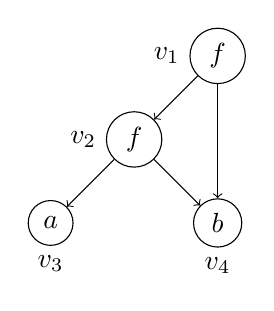
\begin{tikzpicture}[node distance={15mm}, main/.style = {draw, circle}]
\node[main, label=left:$v_{1}$] (1) {$f$};
\node[main, label=left:$v_{2}$] (2) [below left of=1] {$f$};
\node[main, label=below:$v_{3}$] (3) [below left of=2] {$a$};
\node[main, label=below:$v_{4}$] (4) [below right of=2] {$b$};
\draw[->] (1) -- (2);
\draw[->] (2) -- (3);
\draw[->] (2) -- (4);
\draw[->] (1) -- (4);
\end{tikzpicture}
\end{figure}

For a vertex $v$, we will denote by $\lambda(v)$ its label, $\delta(v)$ its outdegree and $Child(v, i)$ its $i$-th child.

Next, we will keep a data structure that is capable of representing a set of disjoint sets of vertices. Each one of these disjoint sets represents a class in an equivalence relation, where every vertex in the same class is known to be equal. This data structure must also be able to check whether two vertices are on the same class and to join two classes. An example of structure with such capabilities is~\cite{union_find}.

Initially, each term is only equal to itself. Then, for each equality $t_{1} = t_{2}$ in $S$ we will use the procedure \textit{MergeCong} presented in figure~\ref{merge_cong} to merge the vertices $v_{1}$ and $v_{2}$ that correspond to $t_{1}$ and $t_{2}$.
Notice that, when we process an equality $t_{1} = t_{2}$, we also have to propagate this information to any other terms that are using $t_{1}$ and $t_{2}$ as parameters (e.g.~if we have $f(t_{1})$ and $f(t_{2})$ as terms, we must also merge their classes). That's why we recursively call \textit{MergeCong} on line 11.
This method has an auxiliary procedure for checking whether two vertices are congruent given the current state. Figure~\ref{cong_cond} shows an implementation of this method, which essentially just checks the premise of Theorem~\ref{cong_theorem}.

\begin{figure}[t]
\begin{algorithmic}[1]
  \Function{IsCongruent}{$v_{1}$, $v_{2}$}
  \If{$\lambda(v_{1}) \neq \lambda(v_{2})$ or $\delta(v_{1}) \neq \delta(v_{2})$}
    \State\Return~$false$
  \EndIf
  \For{$i = 1$ to $\delta(v_{1})$}
  \If{$\neg$ \Call{SameClasses}{\Call{Child}{$v_{1}$, $i$}, \Call{Child}{$v_{2}$, $i$}}}
      \State\Return $false$
    \EndIf
  \EndFor
  \State\Return $true$
  \EndFunction
\end{algorithmic}
\caption{Check Congruence Condition}~\label{cong_cond}
\end{figure}


Once this process is done, we can check whether any pair of terms $t_{1}$ and $t_{2}$ is currently equal to each other by checking whether their corresponding vertices $v_{1}$ and $v_{2}$ are on the same equivalence class (i.e.\ checking whether $Find(v_{1}) = Find(v_{2})$). Therefore, we can use this fact to solve our original problem of checking if the equality $e$ follows from the conjunction of the equalities in $S$.

\subsubsection{Linear Arithmetic}

The second theory that we will be interested in this work is the theory of Linear Arithmetic. A term in this theory is an expression of the form:
\begin{center}
  $\mathlarger{\sum}_{i = 1}^{n} a_{i} x_{i} \bowtie b$
\end{center}

Where each $a_{i}$ and $b$ are constants ranging over rationals, each $x_{i}$ is a variable and $\bowtie$ is one of $\le$, $<$ or $\simeq$ (we model $\ge$ and $>$ as the negation of $<$ and $\le$). If we allow variables to range only over integers, we have the Linear Integer Arithmetic theory, which was described in terms of MSFOL in Example~\ref{ex:lia}. If variables can range over rationals, the corresponding theory is known as Linear Real Arithmetic (LRA), which can be described using MSFOL a similar way.

We will now review the method presented in~\cite{simplex_dpllt} for checking whether a given set of atoms from LRA is satisfiable. The paper also presents an extension of this method for LIA, which we will not show here.

The first step is to, for each atom $t_{i} \bowtie b_{i} \in \phi$ in which $t_{i}$ is a sum of at least two variables, create a fresh variable $s_{i}$. Then, we will define two new sets of atoms: $\phi_{A}$, such that it's atoms are all of the form $s_{i} = t_{i}$, that is, they state the equality between the new variables and the corresponding terms, and $\phi'$, that has all the atoms in $\phi$ but with each term $t_{i}$ substituted by the corresponding $s_{i}$. For instance, let the set of atoms be
$\phi := \{x - y \ge 3, x - 2y < 6, x - y \le 10, x \ge 5\}$.  From this, we would define $\phi_{A} := \{s_{1} = x - y, s_{2} = x - 2y\}$ and $\phi' := \{s_{1} \ge 3, s_{2} < 6, s_{1} \le 10, x \ge 5\}$. It is easy to see that $\phi$ and $\phi_{A} \wedge \phi'$ are equisatisfiable.

Next we will represent the restrictions in $\phi_{A}$ as $Ax = 0$, where $A$ is a matrix and $x$ is a vector with all the variables in the problem (including the ones we added). We will refer to the entry in the $i$-th row and $j$-th column of $A$ as $a_{ij}$. If the original problem had $n$ variables and we added $m$ fresh ones, the matrix $A$ will have $m$ rows and $m + n$ columns. In our example, we would have the following:

\begin{center}
$
A :=
\begin{bmatrix}
  -1 & 1 & 1 & 0 \\
  -1 & 2 & 0 & 1
\end{bmatrix}
x :=
\begin{bmatrix}
  x & y & s_{1} & s_{2}
\end{bmatrix}^{T}
$
\end{center}

\begin{figure}[t]
\begin{algorithmic}[1]
  \Procedure{Update}{$v_{i}$, $val$}
  \For{$v_{j} \in \mathcal{B}$}
    \State $\beta(v_{j}) \gets \beta(v_{j}) + a_{ji}(v - \beta(v_{i}))$
  \EndFor
    \State $\beta(v_{i}) \gets val$
  \EndProcedure
\end{algorithmic}
\caption{Change value of non-basic variable and update all basic variables}
\end{figure}

Now, our problem is reduced to finding a vector $x$ that satisfies $Ax = 0$ and respects all restrictions in $\phi'$, which are all of the form $v_{i} \bowtie b_{i}$. We will assume that there is no strict inequalities in $\phi'$. For an extension of the method presented here for strict inequalities, consult~\cite{simplex_dpllt}. Notice that in this case we can represent the restrictions in $\phi'$ as two sequences of coefficients $l_{i}$ and $r_{i}$, representing a sequence of restrictions of the form $l_{i} \le v_{i} \le r_{i}$, as long as we allow $l_{i}$ to be $-\infty$ in case there is no lower restriction on $v_{i}$ and $r_{i}$ to be $+\infty$ in case there is no upper restriction on $v_{i}$.

We will solve this problem by processing each restriction in $\phi'$ incrementally. Our algorithm will maintain a state that includes the coefficients $l_{i}$ and $r_{i}$, as well as a function $\beta(v)$ that assigns a rational value to each variable $v$. At the beginning, since we haven't processed any inequality yet, we will set each $l_{i}$ to $-\infty$, each $r_{i}$ to $+\infty$, and $\beta(v_{i})$ to $0$ for all $v_{i}$. Additionally, we will keep track of two sets of variables: $\mathcal{N}$ (non-basic variables) and $\mathcal{B}$ (basic variables). Initially, $\mathcal{B}$ will consist of all the variables we added to the problem (each $s_{i}$), while $\mathcal{N}$ will include all the original variables.
Those sets can exchange elements during the execution of the algorithm, but we will always maintain the invariant that all non-basic variables respect their restrictions, that is, $l_{i} \le \beta(v_{i}) \le r_{i}$ for all $v_{i} \in \mathcal{N}$. Also, everytime we update the value of a variable we will also update the values of all basic variables, in order to satisfy the equation $Ax = 0$.

For each restriction in $\phi'$ of the form $v_{i} \le b_{i}$ we will run the procedure \textit{AssertUpper} shown below, and for each restriction of the form $v_{i} \ge b_{i}$ we will run \textit{AssertLower}. If there is a restriction of the form $v_{i} = b_{i}$ we will run both procedures.

\algnewcommand{\IIf}[1]{\State\algorithmicif\ #1\ \algorithmicthen}
\algnewcommand{\EndIIf}{\unskip\ \algorithmicend\ \algorithmicif}

\begin{figure}[t]
\begin{algorithmic}[1]
  \Function{AssertLower}{$v_{i}$, $b_{i}$}
  \IIf{$b_{i} \le l_{i}$} \Return $true$ \EndIIf
  \IIf{$b_{i} > u_{i}$} \Return~$false$ \EndIIf
  \State $l_{i} \gets b_{i}$
  \If{$v_{i}$ is a non-basic variable and $\beta(v_{i}) > u_{i}$}
    \State \Call{Update}{$v_{i}$, $u_{i}$}
  \EndIf
  \State \Return~$true$
  \EndFunction
\end{algorithmic}
\begin{algorithmic}[1]
  \Function{AssertUpper}{$v_{i}$, $b_{i}$}
  \IIf{$b_{i} \ge u_{i}$} \Return $true$ \EndIIf
  \IIf{$b_{i} < l_{i}$} \Return~$false$ \EndIIf
  \State $u_{i} \gets b_{i}$
  \If{$v_{i}$ is a non-basic variable and $\beta(v_{i}) < l_{i}$}
    \State \Call{Update}{$v_{i}$, $l_{i}$}
  \EndIf
  \State \Return~$true$
  \EndFunction
\end{algorithmic}
\caption{Assert inequalities}
\end{figure}

Both functions return $false$ if and only if the current restriction is incompatible with the previous ones, otherwise they correctly update the bounds on the variable on the restriction, and also update its value in case it is a non-basic variable (remember that we keep the invariant that non-basic variables respect their bounds). If the current restriction is $v_{i} \le b_{i}$, we first have to check if the current limit on $v_{i}$ already satisfies this restriction, which is done in line 2 of the function \textit{AssertUpper} and simply return $true$ if this is the case. Otherwise, we compare the current lower bound on $v_{i}$ with $b_{i}$ and immediately return $false$ if it is not, since in this case it would be impossible to find a valid value for $v_{i}$. Finally, if none of these conditions held, we update the limit $u_{i}$ accordingly in line 8 and update the value of $v_{i}$ and of all basic variables in line 10, if it is necessary. The procedure \textit{AssertLower} is symmetrical.


\begin{figure}[t]
\begin{algorithmic}[1]
  \Procedure{PivotAndUpdate}{$v_{i}$, $v_{j}$, $val$}
    \State $\delta \gets \frac{val - \beta(v_{i})}{a_{ij}}$
    \State $\beta(v_{i}) \gets val$
    \State $\beta(v_{j}) \gets \beta(v_{j}) + \delta$
    \For{$v_{k} \in \mathcal{B} \setminus \{v_{i}\}$}
      \State~$\beta(v_{k}) \gets \beta(v_{k}) + a_{kj}\delta$
    \EndFor
    \State $\mathcal{B} \gets (\mathcal{B} \setminus \{v_{i}\}) \cup \{v_{j}\}$
    \State $\mathcal{N} \gets (\mathcal{N} \setminus \{v_{j}\}) \cup \{v_{i}\}$
  \EndProcedure
\end{algorithmic}
\caption{Update and pivot basic with non-basic variable}
\end{figure}

Lastly, if it was possible to run the assertion procedures on all the inequalities from the input without any of them returning \textit{false}, we run the procedure \textit{Check} presented in figure~\ref{check_lra}. The goal of this function is to manipulate the values of the non-basic variables until all variables respect their restrictions, or report that it is impossible, and, therefore, the original formula is unsatisfiable. The first step it takes, in line 2 is to select a variable $v_{i} \in \mathcal{B}$ that is violating its bounds. If there is no such variable then all restrictions are satisfied, and it can just return \textit{true}, as is done in line 4. If $\beta(v_{i}) < l_{i}$, then we must find a non-basic variable $v_{j}$ such that we can modify it without violating its restrictions in a way that the value of $v_{i}$ will increase. If $a_{ij}$ is positive, increasing $v_{j}$ will also increase $v_{i}$, therefore, in order to use $v_{j}$ we need $\beta(v_{j}) < u_{j}$. Similarly, if $a_{ij}$ is negative, we would need $\beta(v_{j}) > l_{j}$. If there is no suitable variable, then it's impossible increase the value of $v_{i}$, therefore the problem is unsatisfiable. This condition is checked on lines 9 and 16. Otherwise, we can find such $v_{j}$. In this case, we set the value of $v_{j}$ to the appropriate limit and make $v_{i}$ a non-basic variable and $v_{j}$ a non-basic variable with the procedure \textit{PivotAndUpdate} in lines 12 and 19. After this, we repeat the process until all restrictions were satisfied. The case where $\beta(v_{i}) > u_{i}$ is symmetrical. In~\cite{simplex_dpllt}, the authors prove that this method always terminates and returns \textit{true} if and only if the original problem was satisfiable.

\begin{figure}[t]
\begin{algorithmic}[1]
  \Function{Check}{\null}
    \State Let $v_{i}$ be the basic variable that violates a restriction with the smallest index.
    \If{There is no such $v_{i}$}
      \State \Return{$true$}
    \EndIf
    \If{$\beta(v_{i}) < l_{i}$}
      \State Let $v_{j}$ be the non-basic variable with smallest index such that\\
      \qquad \qquad $(a_{ij} > 0 \wedge \beta(v_{j}) < u_{j}) \vee (a_{ij} < 0 \wedge \beta(v_{j}) > l_{j})$
      \If{There is no such $v_{j}$}
        \State \Return{$false$}
      \EndIf
      \State \Call{PivotAndUpdate}{$v_{i}$, $v_{j}$, $l_{i}$}
    \ElsIf{$\beta(v_{i}) > u_{i}$}
        \State Let $v_{j}$ be the non-basic variable with smallest index such that\\
        \qquad \qquad $(a_{ij} < 0 \wedge \beta(v_{j}) < u_{j}) \vee (a_{ij} > 0 \wedge \beta(v_{j}) > l_{j})$
        \If{There is no such $v_{j}$}
          \State \Return{$false$}
        \EndIf
        \State \Call{PivotAndUpdate}{$v_{i}$, $v_{j}$, $u_{i}$}
    \EndIf
    \State \Call{Check}{\null}
  \EndFunction

\end{algorithmic}
\caption{Check if it's possible to satisfy all restrictions}\label{check_lra}
\end{figure}

\subsection{Proof Certificates}\label{sec:proof_cert}

In order to convince the ITP that the result found by the SMT solver is correct, we need some sort of evidence provided by the ATP.
We will refer to these evidences as proof certificates. The main feature of a good certificate is being easy to check if they are really sufficient to prove the desired result. In particular, it must be easier to check a certificate then to solve the original problem. The theories that are of our interest in this project have already been instrumentized in cvc5 so that the solver can produce proof certificates for them. In this section we present the formats of these certificates.

\subsubsection{Certificates for Boolean Satisfiability}

First, let's consider what would be suitable certificates for results for the SAT problem. If the SMT solver determines that a given instance is satisfiable, then a certificate could be simply the valuation of the variables in the problem. One could verify that the certificate is valid simply by replacing the valuation on the original formula and checking if it evaluates to \textit{true}. For unsatisfiability results, there is not a certificate that is so simple. The alternative mainly used by SMT solvers is to produce a \textit{resolution tree}. A resolution tree is a binary tree in which each leaf correspond to a clause from the SAT instance, each internal node correspond to the clause resulting of applying Theorem~\ref{res_theorem} on its two children and the root correspond to the empty clause.

For instance\footnote{Example taken from~\cite{smtcoq}}, for the SAT formula that corresponds to the conjunction of the set of clauses $\{x \vee y, x \vee \neg y \vee z, \neg x \vee z,  \neg z\}$, a possible resolution tree that certificates its unsatisfiability is the following:

\inferLineSkip=3pt
\[
\infer[]{\bot}{
  \infer[]
  {x}
  {x \vee y & \infer[]{x \vee \neg y}{x \vee \neg y \vee z & \neg z}} & \infer[]{\neg x}{\neg x \vee z & \neg z}}
\]

In order to check it, it's enough to check if the leafs correspond to premisses, each resolution was applied correctly and the root corresponds to the empty clause. It is known that, for any unsatisfiable instance of the SAT problem, there exists at least one resolution tree that certificates its unsatisfiability~\cite{res_tree_complete}. This is the format produced by cvc5 and, therefore, we will use it in this thesis.

\subsubsection{Certificates for Congruence Closure}

Remember that, in the theory of Equality and Uninterpreted Functions, we are given a set of equalities and inequalities involving variables and functions and we must check whether they are satisfiable. Similarly to the previous case, a suitable proof certificate for a positive result is a valuation of the variables in the problem, which can be trivially checked. If the set of atoms is unsatisfiable, then we can build a proof tree, similar to the resolution tree presented before. The only difference is that, instead of using the resolution theorem to infer new propositions, this tree will use the axioms that equality satisfies (reflexivity, symmetry and transitivity), as well as Theorem~\ref{cong_theorem}. For instance, consider the following set of propositions: $\{a \simeq f(f(a)), a \simeq f(f(f(a))), f(a) \not\simeq a\}$. One possible proof tree that certificates its unsatisfiability is the following:

\[
  \infer[]{\bot}{\infer[trans]{f(a) \simeq a}{\infer[cong]{f(a) \simeq f(f(f(a)))}{a \simeq f(f(a))} & \infer[symm]{f(f(f(a))) \simeq a}{a \simeq f(f(f(a)))}} & f(a) \not\simeq a}
\]

\subsubsection{Certificates for Linear Arithmetic}

The proof certificates for unsatisfiability of problems on the theory of linear arithmetic rely on the following variant of Farkas' lemma~\cite{farkas_ref}:

\begin{theorem}[Farkas' Lemma]\label{farkas_lemma}
  Let $C$ be a sequence of $m$ restrictions, where the $j$-th one has the form $\mathlarger{\sum}_{i = 1}^{n} a_{i} x_{i} \bowtie_{j} b_{j}$ and each $\bowtie_{j}$ is either $\le$ or $<$. If there is no solution for the conjunction of these restrictions, then there exists a sequence of positive coefficients $s_{i}$, known as Farkas' coefficients, that satisfies $\mathlarger{\sum}_{i = 1}^{m} s_{i} (\mathlarger{\sum}_{j = 1}^{n} a_{j} x_{j}) = 0$ and $\mathlarger{\sum}_{i = 1}^{m} s_{i} b_{i} \bowtie 0$, where $\bowtie$ is $\le$ if any of the original relation symbols was strict or $<$ otherwise.
\end{theorem}

One can use a sequence of coefficients with these properties to certify that a given instance of the problem is unsatisfiable. Given the sequence $s$, we can multiply each one of the restrictions $\sum_{i = 1}^{n} a_{i} x_{i} \bowtie_{j} b_{j}$ by $s_{j}$, obtaining $ s_{j} \sum_{i = 1}^{n} a_{i} x_{i} \bowtie_{j} s_{j} b_{j}$ (note that $\bowtie$ does not change, as $s_{j}$ is positive). Adding all the restrictions we get $\sum_{j = 1}^{m} s_{j} (\sum_{i = 1}^{n} a_{i} x_{i}) \bowtie^{*} \sum_{j = 1}^{m} s_{j} b_{j}$, where $\bowtie^{*}$ is $<$ if at least one $\bowtie_{j}$ was $<$ or $\le$ otherwise. By hypothesis, the left-hand side evaluates to $0$. If $\bowtie^{*}$ is $<$, then the right-hand side is smaller then or equal to $0$, which is an absurd. If $\bowtie^{*}$ is $\le$, then the right hand side is positive, which is also an absurd ($0 < 0$). Therefore, in order to verify that a given sequence of coefficients indeed prove that the restrictions are unsatisfiable, it's sufficient to apply the rules stating that we can add inequalities and multiply them by constants in the way we did, and then evaluate the final inequality to obtain a contradiction.

Since it is always possible to find these coefficients for unsatisfiable instances of the problem, the SMT solver can provide them as a proof certificate for this theory. Indeed, this is the certificate used by cvc5, and it is the one we will be interested in this thesis.
% Using this fact, an SMT solver can compute the Farkas' coefficients
% Using this fact, it's enough to provide the Farkas' coefficients to certificate the unsatisfability of an instance of the problem.


\subsection{Example of Application}

Given a program and a formal specification of some property related to the program, it is often the case that we can express the proposition that asserts the correctness of the program with respect to that property as an SMT instance. For instance, consider the well known \texttt{abs} function, that takes an integer and returns its absolute value. The usual way to implement it is through a branch that checks whether the input variable is positive or negative. In case it is positive, its own value is returned. Otherwise, the value multiplied by $-1$ is returned. This implementation
is presented in Figure~\ref{originalAbs}.

\begin{figure}
\begin{algorithmic}[1]
\Function{abs}{x}
\If{$x < 0$}
  \State\Return$-x$
\Else
  \State\Return$x$
\EndIf
\EndFunction
\end{algorithmic}
\caption{Original implementation of the absolute value function}\label{originalAbs}
\end{figure}

In program analysis, it is quite useful to eliminate branches from programs since this action completely removes one possible path that the flow of the program can take, simplifying it's analysis (besides optimizing it's performance). Obviously, this must be done with caution to not modify the original behavior of the program. In his book~\cite{hacker_delight}, Henry Warren proposes a branchless implementation of the \texttt{abs} function, which is presented in Figure~\ref{branchlessAbs}. The symbol $\bigoplus$ represents the bitwise \textit{xor} operation.

\begin{figure}[t]
\begin{algorithmic}[1]
\Function{abs'}{x}
  \State $y \gets x >> 31$
  \State \Return $(x \bigoplus y) - y$
\EndFunction
\end{algorithmic}\label{branchlessAbs}
\caption{Branchless implementation of the absolute value function}
\end{figure}

We can design an instance of the SMT problem that asserts that both implementations produce the same output, when given the same input. We present the instance written in SMT-Lib~\cite{smtlib}, a standardized syntax for representing SMT problems, in Figure~\ref{smtlib_branchless}.

\begin{figure}[t]
\begin{minted}[linenos]{smtlib2.py -x}
(set-logic QF_BV)
(declare-const x (_ BitVec 32))
(declare-const result1 (_ BitVec 32))
(assert (= result1 (ite (bvslt x #x00000000) (bvneg x) x)))
(declare-const y (_ BitVec 32))
(declare-const result2 (_ BitVec 32))
(assert (= y (bvashr x (_ bv31 32))))
(assert (= result2 (bvsub (bvxor x y) y)))
(assert (distinct result1 result2))
(check-sat)
\end{minted}
\caption{SMT-Lib script for equivalence of absolute functions}\label{smtlib_branchless}
\end{figure}


First, in line 1, we set the combination of theories that will be used in this problem. In our case, we will be using \textit{QF\_BV}, which stands for quantifier free bitvectors. This means that this instance of the problem is not allowed to use quantifiers and is allowed to declare and use variables living in the Bitvector sort, as well as operations over this sort. Bitvectors are fixed-length arrays of bits. They are useful for representing machine integers, as they can simulate their semantics.

Next, in lines 2 and 3, we define two constants, both from the sort \textit{BitVec 32} (arrays of 32 bits): \textit{x} and \textit{result1}. The first one represents the input value from the original \textit{abs} function, and the second one, the result produced by that function. We then have to add an assertion in line 4 that binds the variable \textit{result1} to the output of the function \textit{abs} in terms of \textit{x}. We translate the branch from the pseudocode as the \textit{ite} operator, the comparison as the \textit{bvslt} operator and the multiplication by -1 as the \textit{bvneg} operation. In lines 5 to 8 we repeat the process to define \textit{y} and \textit{result2}, which corresponds to the result of the branchless \textit{abs} function. Finally, we assert that \textit{result1} and \textit{result2} must be different in line 9. If this problem is satisfiable, then there is a value for \textit{x} which produces different values in each function. If it is unsatisfiable, then we can be sure that no such value exists, therefore, both functions are equivalent. Note that we are not verifying that the actual code of the functions are equivalent, just an abstraction over it's implementation.

% Given that we have very efficient systems to solve such problems, which will be introduced later, the possibility of formally verifying programs using this technology is quite promising. Indeed, \tom{pegar referencias do paper do leonardo (https://fm.csl.sri.com/SSFT14/smt-application-chapter.pdf)}
%

% \begin{itemize}
%   \item revolucao sat
%   \item representar propriedades de programas como problemas smt
%   \item geracao de casos de teste
%   \item geracao de programas
%   \item F*, Dafny
% \end{itemize}
